%
%===============>>  ГРУППА 11-1 МОДУЛЬ 5  <<=============
%
\setmodule{5}

%BEGIN_FOLD % ====>>_____ Занятие 1 _____<<====
\begin{class}[number=1]
	\begin{listofex}
		\item Занятие 1
	\end{listofex}
\end{class}
%END_FOLD

%BEGIN_FOLD % ====>>_____ Занятие 2 _____<<====
\begin{class}[number=2]
	\begin{listofex}
		%1
		\item Материальная точка движется прямолинейно по закону \(x(t) = 6t^2 - 48t + 17\) (где \(x\)  — расстояние от точки отсчета в метрах, \(t\)  — время в секундах, измеренное с начала движения). Найдите ее скорость (в м/с) в момент времени \(t  =  9\) с.
		%2
		\item Материальная точка движется прямолинейно по закону \(x(t) = -t^4 + 6t^3 + 5t + 23\) (где \(x\)  — расстояние от точки отсчета в метрах, \(t\)  — время в секундах, измеренное с начала движения). Найдите ее скорость в (м/с) в момент времени \(t = 3\) с.
		%3
		\item
		\begin{minipage}[t]{\bodywidth}
			На рисунке изображен график функции \( y = f(x)\), определенной на интервале \((-5; 5)\). Найдите количество точек, в которых касательная к графику функции параллельна прямой \(y  =  6\) или совпадает с ней.
		\end{minipage}
		\hspace{0.02\linewidth}
		\begin{minipage}[t]{\picwidth}
			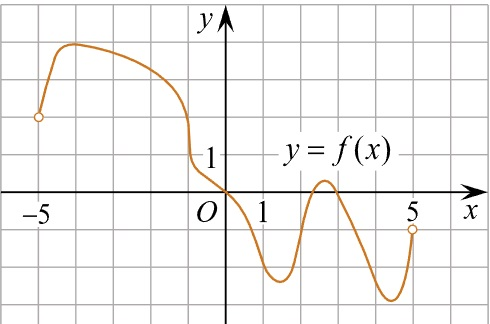
\includegraphics[align=t, width=\linewidth]{\picpath/G111M5L2-1}
		\end{minipage}
		%4
		\item
		\begin{minipage}[t]{\bodywidth}
			На рисунке изображен график производной функции \(f(x)\), определенной на интервале \((-10; 2)\). Найдите количество точек, в которых касательная к графику функции \(f(x)\) параллельна прямой \(y = -2x - 11\) или совпадает с ней.
		\end{minipage}
		\hspace{0.02\linewidth}
		\begin{minipage}[t]{\picwidth}
			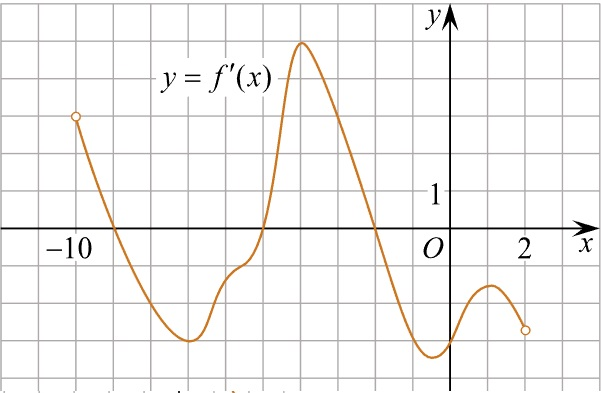
\includegraphics[align=t, width=\linewidth]{\picpath/G111M5L2-2}
		\end{minipage}
		%5
		\item
		\begin{minipage}[t]{\bodywidth}
			На рисунке изображен график производной функции \(f(x)\) , определенной на интервале \( (-6;6) \) . Найдите промежутки возрастания функции \(f(x)\) . В ответе укажите сумму целых точек, входящих в эти промежутки.
		\end{minipage}
		\hspace{0.02\linewidth}
		\begin{minipage}[t]{\picwidth}
			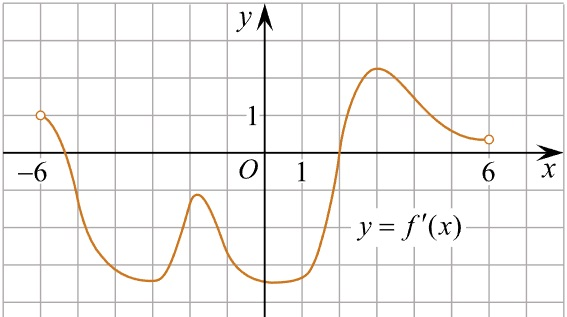
\includegraphics[align=t, width=\linewidth]{\picpath/G111M5L2-3}
		\end{minipage}
		%6
		\item
		\begin{minipage}[t]{\bodywidth}
			На рисунке изображен график функции \(y = f(x)\), определенной на интервале \((-6; 8)\). Определите количество целых точек, в которых производная функции положительна.
		\end{minipage}
		\hspace{0.02\linewidth}
		\begin{minipage}[t]{\picwidth}
			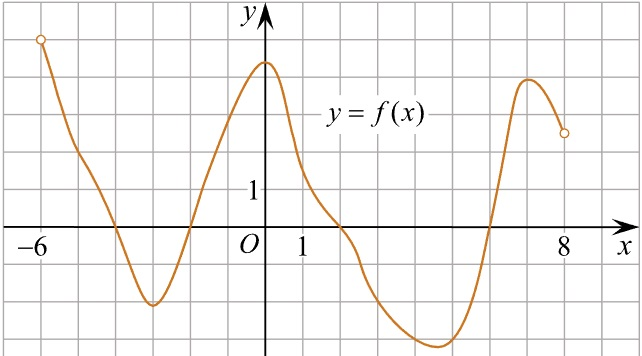
\includegraphics[align=t, width=\linewidth]{\picpath/G111M5L2-4}
		\end{minipage}
		%7
		\item Найдите:
		\begin{itasks}[1]
			\task точку максимума функции \(y = x^3 - 48 + 17\)
			\task наименьшее значение функции \(y = x^3 - 27x\) на отрезке \([0;4]\)
			\task точку максимума функции \(y = x^3 - 5x^2 + 7x -5\)
			\task точку максимума функции \(y = -\dfrac{x^2+289}{x}\)
			\task наименьшее значение функции \(y = \dfrac{x^2+25}{x}\) на отрезке \([1;10]\)
		\end{itasks}
	\end{listofex}
\end{class}
%END_FOLD

%BEGIN_FOLD % ====>>_____ Занятие 3 _____<<====
\begin{class}[number=3]
	\begin{listofex}
		\item Занятие 3
	\end{listofex}
\end{class}
%END_FOLD

%BEGIN_FOLD % ====>>_____ Занятие 4 _____<<====
\begin{class}[number=4]
	\begin{listofex}
		\item Занятие 4
	\end{listofex}
\end{class}
%END_FOLD

%BEGIN_FOLD % ====>>_____ Занятие 5 _____<<====
\begin{class}[number=5]
	\begin{listofex}
		\item Занятие 5
	\end{listofex}
\end{class}
%END_FOLD

%BEGIN_FOLD % ====>>_____ Занятие 6 _____<<====
\begin{class}[number=6]
	\begin{listofex}
		\item Занятие 6
	\end{listofex}
\end{class}
%END_FOLD

%BEGIN_FOLD % ====>>_____ Занятие 7 _____<<====
\begin{class}[number=7]
	\begin{listofex}
		\item Занятие 7
	\end{listofex}
\end{class}
%END_FOLD

%BEGIN_FOLD % ====>>_ Домашняя работа 1 _<<====
\begin{homework}[number=1]
	\begin{listofex}
		\item ДЗ 1
	\end{listofex}
\end{homework}
%END_FOLD

%BEGIN_FOLD % ====>>_ Домашняя работа 2 _<<====
\begin{homework}[number=2]
	\begin{listofex}
		\item ДЗ 2
	\end{listofex}
\end{homework}
%END_FOLD

%BEGIN_FOLD % ====>>_ Домашняя работа 3 _<<====
\begin{homework}[number=3]
	\begin{listofex}
		\item ДЗ 3
	\end{listofex}
\end{homework}
%END_FOLD

%BEGIN_FOLD % ====>>_ Проверочная работа _<<====
\begin{exam}
	\begin{listofex}
		\item Проверочная работа
	\end{listofex}
\end{exam}
%END_FOLD
